% ============================================================================
% Week 7 -- LECTURE NOTE (student-facing)
%
% Alternative formulations (moved here from week06-note.tex to match the
% schedule). Branch-and-bound §4-6 ported from integer-programming-course
% lecture-notes/week06.tex §4-6. Style of week05-note.tex. Self-contained.
% ============================================================================
\documentclass[10pt]{article}

\usepackage[a4paper, margin=1.5cm]{geometry}
\usepackage{amsmath, amssymb}
\usepackage[dvipsnames]{xcolor}
\usepackage{graphicx}
\usepackage{array}
\usepackage{tikz}
\usetikzlibrary{matrix}
\usepackage{needspace}
\usepackage[hidelinks]{hyperref}

\definecolor{ruleink}{RGB}{18, 68, 140}
\definecolor{demoink}{RGB}{140, 82, 20}
\definecolor{keyink}{RGB}{20, 90, 20}
\definecolor{watchink}{RGB}{86, 60, 140}
\definecolor{punchink}{RGB}{170, 30, 60}

\setlength{\parindent}{0pt}
\pagestyle{empty}
\frenchspacing

% tighter spacing around centered displays
\AtBeginDocument{%
  \abovedisplayskip=4pt plus 1pt
  \belowdisplayskip=4pt plus 1pt
  \abovedisplayshortskip=2pt
  \belowdisplayshortskip=2pt}

% ---- one section -----------------------------------------------------------
\newcommand{\beat}[2]{%   number, title
  \par\medskip\needspace{8\baselineskip}%   never strand a title at the page foot
  {\color{ruleink}\rule{\textwidth}{1pt}}\par\nobreak\vspace{2pt}
  {\large\bfseries #1.\; #2}\par\nobreak\vspace{3pt}}

% ---- board content ---------------------------------------------------------
\newenvironment{board}{%
  \par\vspace{2pt}
  \begingroup\leftskip=1.3em\relax}{%
  \par\endgroup\vspace{2pt}}

% ---- highlights ------------------------------------------------------------
\newcommand{\demo}[2]{\par{\leavevmode\color{demoink}\small\textbf{demo}\quad\texttt{#1} --- #2}\par}
\newcommand{\watch}[1]{\par{\color{watchink}\small\textbf{watch}\quad #1}\par}
\newcommand{\key}[1]{\par\vspace{1pt}{\color{keyink}\small\textbf{KEY}\quad\textbf{#1}}\par}
\newcommand{\takeaway}[1]{%
  \par\vspace{2pt}\noindent
  {\color{punchink}\rule{2pt}{10pt}}\;{\color{punchink}\small\textbf{takeaway}\quad\textbf{#1}}\par\vspace{2pt}}

% ---- proof sketch ----------------------------------------------------------
\newenvironment{sketch}{%
  \par\vspace{5pt}
  \begingroup\advance\leftskip by 1.3em\relax
  \textit{Proof sketch.}\ }{%
  {\unskip\nobreak\hfil\penalty50\hskip1em\hbox{}\nobreak\hfil$\square$%
   \parfillskip=0pt\finalhyphendemerits=0\par}\endgroup\vspace{5pt}}

\begin{document}

{\Large\bfseries Week 7 --- Alternative Formulations, and Branch-and-Bound}\\[2pt]
{\small OL7014 Integer Programming \quad\textbullet\quad Instructor: Prof.\ H.\ Park \quad\textbullet\quad Week of Oct 5, 2026}

% ---------------------------------------------------------------- 1
\beat{1}{Alternative formulations --- one $X$, many $P$}
\begin{board}
remember from week 5 --- the \textbf{LP relaxation}:
\[
  z_{\mathrm{IP}} \;=\; \max_{x} \{\, c^{\top}x : Ax \le b, \ x \in \mathbb{Z}^n_{+} \,\}
  \quad\;\le\;\quad
  z_{\mathrm{LPR}} \;=\; \max_{x} \{\, c^{\top}x : Ax \le b, \ x \ge 0 \,\}
\]
let $P = \{x \in \mathbb{R}^n_{+} : Ax \le b\}$ and $X = P \cap \mathbb{Z}^n$; \ then
\[
  z_{\mathrm{IP}} \;=\; \max_{x} \{\, c^{\top}x : x \in X \,\}
  \quad\;\le\;\quad
  z_{\mathrm{LPR}} \;=\; \max_{x} \{\, c^{\top}x : x \in P \,\}
\]

\textbf{Def.} \ a polyhedron $P = \{x \in \mathbb{R}^n_{+} : Ax \le b\}$ is a \textbf{formulation} for $X$ \ iff \ $X = P \cap \mathbb{Z}^n$
\vspace{1pt}

\quad $X$ = the feasible integer points --- $P$ must contain \emph{exactly} $X$, not more, not less
\vspace{3pt}

there can be many \textbf{alternative formulations} $P$ for $X$
\vspace{2pt}

\textbf{example} (Knapsack problem with three items):
\[
  X = \bigl\{\, (0,0,0),\ (1,0,0),\ (0,1,0),\ (0,0,1) \,\bigr\} \ \subset \ \mathbb{Z}^3
\]
\begin{center}
\begin{tabular}{@{}l|l|l@{}}
 $P_1 = \{x \in \mathbb{R}^3_{+} : A^1 x \le b^1\}$ & $3x + 3y + 3z \le 5$ & $A^1 = \begin{bmatrix} 3 & 3 & 3 \end{bmatrix}, \ \ b^1 = 5$ \\[4pt] \hline
 \rule{0pt}{22pt}%
 $P_2 = \{x \in \mathbb{R}^3_{+} : A^2 x \le b^2\}$ & $\begin{array}{@{}c@{}c@{}c@{}c@{}c@{}l@{}}
            x & {}+{} & y &       &   & {}\le 1 \\
            x &       &   & {}+{} & z & {}\le 1 \\
              &       & y & {}+{} & z & {}\le 1
          \end{array}$
       & $A^2 = \begin{bmatrix} 1 & 1 & 0 \\ 1 & 0 & 1 \\ 0 & 1 & 1 \end{bmatrix}, \ \ b^2 = \begin{bmatrix} 1 \\ 1 \\ 1 \end{bmatrix}$ \\[14pt]
\end{tabular}
\end{center}
both contain exactly $X$: \ $P_1 \cap \mathbb{Z}^3 = P_2 \cap \mathbb{Z}^3 = X$ --- \textbf{alternative formulations};
the polyhedra $P_1, P_2$ themselves are \emph{different}
\vspace{2pt}

different formulations $P_1$ and $P_2$ may lead to different upper-bound quality
\vspace{2pt}

let $c = (1,1,1)$; \ hence $x^{*}_{\mathrm{IP}} = (1,0,0)$ (or any unit vector) and $z_{\mathrm{IP}} = c^{\top}x^{*}_{\mathrm{IP}} = 1$
\vspace{1pt}

\quad over $P_1$: \ $x^{*}_{\mathrm{LPR}} = (5/3,0,0)$, \ $z^{1}_{\mathrm{LPR}} = 5/3$
\vspace{1pt}

\quad over $P_2$: \ $x^{*}_{\mathrm{LPR}} = (1/2,1/2,1/2)$, \ $z^{2}_{\mathrm{LPR}} = 3/2$
\[
  z_{\mathrm{IP}} = 1 \;<\; z^{2}_{\mathrm{LPR}} = 3/2 \;<\; z^{1}_{\mathrm{LPR}} = 5/3
\]
$P_2$ gives the tighter bound
\end{board}
\takeaway{this is why modelling is critical in IP: one $X$, many $P$ --- and you chose which one when you wrote the model down.}

% ---------------------------------------------------------------- 2
\beat{2}{Which formulation is better?}
\begin{board}
\textbf{Def.} (Wolsey, Def.~1.5) \ given $X \subseteq \mathbb{Z}^n$ and formulations $P_1, P_2$ for $X$: \
$P_1$ is a \textbf{better} formulation than $P_2$ \ iff \ $P_1 \subset P_2$
\vspace{1pt}

\quad both contain the same integer points; $P_1 \subset P_2$ = less \emph{fractional} junk = an LP relaxation closer to the truth
\vspace{3pt}

\textbf{how to prove $P_1 \subset P_2$} --- $n \le 3$: draw it. \ in general, do the following
\begin{center}
\begin{tabular}{@{}l|l@{}}
 \textbf{step 1} & show every $x \in P_1$ is in $P_2$ \qquad ($P_1 \subseteq P_2$) \\[2pt]
 \textbf{step 2} & exhibit one $\bar{x} \in P_2$ with $\bar{x} \notin P_1$ \qquad (strict) \\
\end{tabular}
\end{center}
if $P_1 = P_2$: \ the two formulations are \textbf{equivalent}
\vspace{1pt}

if $P_1 \setminus P_2$ and $P_2 \setminus P_1$ are both nonempty: \ the two formulations are \textbf{incomparable}
\end{board}
\takeaway{trade-off: a tighter $P$ usually costs more constraints.}

% ---------------------------------------------------------------- 3
\beat{3}{$\operatorname{conv}(X)$ --- the ideal formulation, and the catch}
\begin{board}
\textbf{Def.} \ the \textbf{convex hull} of $X \subseteq \mathbb{R}^n$ is the minimal convex set containing $X$, denoted $\operatorname{conv}(X)$
\vspace{2pt}

\begin{center}
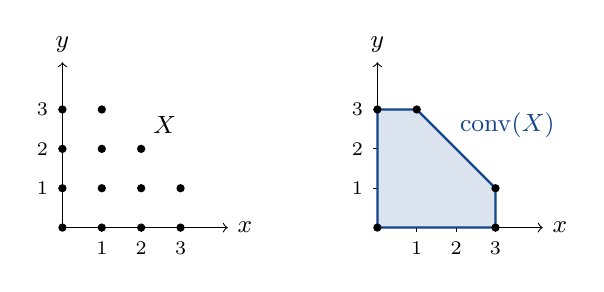
\begin{tikzpicture}[scale=0.5]
  \foreach \s in {0, 8} {
    \begin{scope}[shift={(\s,0)}]
      \draw[->] (0,0) -- (4.2,0) node[right] {\small $x$};
      \draw[->] (0,0) -- (0,4.2) node[above] {\small $y$};
      \foreach \t in {1,2,3} {
        \draw (\t,0) -- (\t,-0.12) node[below] {\scriptsize \t};
        \draw (0,\t) -- (-0.12,\t) node[left] {\scriptsize \t};
      }
    \end{scope}
  }
  % left: X
  \foreach \p in {(0,0),(1,0),(2,0),(3,0),(0,1),(1,1),(2,1),(3,1),(0,2),(1,2),(2,2),(0,3),(1,3)}
    \fill \p circle (3pt);
  \node at (2.6,2.6) {\small $X$};
  % right: conv(X)
  \begin{scope}[shift={(8,0)}]
    \fill[ruleink!15] (0,0) -- (3,0) -- (3,1) -- (1,3) -- (0,3) -- cycle;
    \draw[ruleink, thick] (0,0) -- (3,0) -- (3,1) -- (1,3) -- (0,3) -- cycle;
    \foreach \p in {(0,0),(3,0),(3,1),(1,3),(0,3)}
      \fill \p circle (3pt);
    \node[ruleink] at (3.3,2.6) {\small $\operatorname{conv}(X)$};
  \end{scope}
\end{tikzpicture}
\end{center}

facts, stated without proof:
\begin{center}
\begin{tabular}{@{}l|l@{}}
 1 & $\operatorname{conv}(X)$ is a polyhedron: \ $\operatorname{conv}(X) = \{x \in \mathbb{R}^n_{+} : A^{*}x \le b^{*}\}$
     \ --- so $(A^{*}, b^{*})$ is a formulation for $X$: the \textbf{ideal} one \\[2pt]
 2 & $\operatorname{conv}(X) \subseteq P$ for \emph{every} formulation $P$ of $X$ --- nothing is better \\[2pt]
 3 & $\operatorname{conv}(X)$ has \textbf{integer extreme points} \\
\end{tabular}
\end{center}
\vspace{2pt}

\textbf{ideal reduction of IP to LP:} \ one problem, $\max\{c^{\top}x : x \in X\}$, and two ways to write it down ---
the IP, and the \textbf{convex-hull problem} (CHP), an LP over $\operatorname{conv}(X)$:
\[
  z_{\mathrm{IP}} \;=\; \max_{x} \{\, c^{\top}x : x \in X \,\} \ \ \text{an IP},
  \qquad
  z_{\mathrm{CHP}} \;=\; \max_{x} \{\, c^{\top}x : x \in \operatorname{conv}(X) \,\} \ \ \text{just an LP}
\]
\textbf{Prop.} \ $z_{\mathrm{IP}} = z_{\mathrm{CHP}}$, and an extreme-point optimum of the CHP is an optimum of the IP
\begin{sketch}
a CHP extreme-point optimum $x^{*}_{\mathrm{CHP}}$ is integer (fact 3) $\Rightarrow$ $x^{*}_{\mathrm{CHP}} \in X$: IP-\emph{feasible},
so $z_{\mathrm{CHP}} \le z_{\mathrm{IP}}$; \ and $X \subset \operatorname{conv}(X)$ makes every IP point CHP-feasible, so $z_{\mathrm{IP}} \le z_{\mathrm{CHP}}$
\end{sketch}
so \textbf{you can ignore the integrality constraint}; \ for every other formulation ($P \supsetneq \operatorname{conv}(X)$) we must impose integrality and solve an IP
\vspace{3pt}

\textbf{example} (the $X$ drawn above):
\[
\begin{aligned}[t]
  \max\ & 4x + 5y \\
  \text{s.t.}\ & 3x + y \le 10, \\
  & x + 3y \le 10, \\
  & x, y \ge 0 \ \text{and int}
\end{aligned}
\qquad
\operatorname{conv}(X) \;=\; \bigl\{\, x \ge 0, \ \ y \ge 0, \ \ x \le 3, \ \ y \le 3, \ \ x + y \le 4 \,\bigr\}
\]
\quad the vertices $(0,0), (3,0), (3,1), (1,3), (0,3)$ are all integer, and the CHP returns $(1,3)$,
$z_{\mathrm{CHP}} = 19 = z_{\mathrm{IP}}$ --- an integer answer with no integrality constraint anywhere
\vspace{3pt}

\textbf{the CHP is \emph{not} the LP relaxation:} the relaxation optimizes over $P \supseteq \operatorname{conv}(X)$ and
overshoots; the CHP optimizes over $\operatorname{conv}(X)$ and is exact
\vspace{3pt}

so why is this not the end of the course?
\vspace{1pt}

\quad 1. hard to characterise $\operatorname{conv}(X)$: it may need an \textbf{exponential number} of rows
\vspace{1pt}

\quad 2. even harder: \emph{proving} that what you have is $\operatorname{conv}(X)$
\end{board}
\takeaway{conv($X$) would turn every IP into an LP. we almost never have it. so we do the next best thing: get $P$ as tight as we can afford (\S 2), then pay for the rest with search --- branch \& bound, next.}

% ---------------------------------------------------------------- 4
\beat{4}{Divide and conquer}
\begin{board}
two bounds squeeze $z_{\mathrm{IP}}$ from both sides:
\[
  \underbrace{c^{\top}\hat{x}}_{\hat{x} \in X:\ \text{a feasible plan}}
  \;\;\le\;\; z_{\mathrm{IP}} \;\;\le\;\;
  \underbrace{z_{\mathrm{LPR}}}_{\text{a relaxation (\S 1)}}
\]
the best feasible plan found so far is the \textbf{incumbent} $\hat{x}$, with value $\underline{z} = c^{\top}\hat{x}$ --- the lower bound
\vspace{3pt}

\textbf{Prop.} \ if $X = X_1 \cup \dots \cup X_K$, then $z_{\mathrm{IP}} = \max_j z^j$, \ where $z^j = \max\{c^{\top}x : x \in X_j\}$
--- the best over $X$ is the best of the pieces' bests
\vspace{3pt}

that is the whole idea: chop $X$ into pieces; bound each piece with its LP relaxation; a piece whose bound cannot beat the
incumbent is \emph{thrown away without ever being searched} --- \textbf{implicit enumeration}: every solution accounted for, none visited
\end{board}

% ---------------------------------------------------------------- 5
\beat{5}{Branch \& bound}
\par{\leavevmode\color{demoink}\small\textbf{demo}\quad\texttt{demo6\_branch\_and\_bound.py}}\par
\begin{board}
when can a piece $X_k$ be thrown away? \ its LP relaxation tells you --- three \textbf{prune} rules:
\begin{center}
\begin{tabular}{@{}l|l@{}}
 \textbf{infeasibility} & LP infeasible $\Rightarrow$ $X_k = \emptyset$ \ (it sits inside the LP's feasible set) \\[2pt]
 \textbf{bound}         & $z_{\mathrm{LPR}} \le \underline{z}$ $\Rightarrow$ nothing in $X_k$ beats the incumbent \\[2pt]
 \textbf{optimality}    & $x^{*}_{\mathrm{LPR}}$ integer $\Rightarrow$ it is optimal for $X_k$ \ --- a new incumbent if it beats $\underline{z}$ \\
\end{tabular}
\end{center}
\vspace{2pt}

\textbf{notation.} \ let $P_0 = \{x \in \mathbb{R}^n_{+} : Ax \le b\}$, and similarly $P_k$ for node $k$ of the search tree:
\[
  LP_0: \ \max_{x} \{\, c^{\top}x : x \in P_0 \,\},
  \qquad\qquad
  LP_k: \ \max_{x} \{\, c^{\top}x : x \in P_k \,\}
\]
$LP_0$ is the LP relaxation of the IP; \ $P_k$ is $P_0$ plus the bounds added by branching on the way down to node $k$,
so $LP_k$ relaxes the piece $X_k = P_k \cap \mathbb{Z}^n$
\vspace{1pt}

\quad shorthand: \ $LP_k + \{x_j \le a\}$ = the LP over $P_k \cap \{x : x_j \le a\}$, e.g.\ $LP_1 = LP_0 + \{x \le 2\}$; \
nodes are numbered in the order they are created
\vspace{3pt}

\needspace{20\baselineskip}%   keep the example with its tree
\textbf{example} (week 1's problem --- the $X$ drawn in \S 3):
\[
  \max\; 4x + 5y
  \qquad \text{s.t.} \qquad
  x + 3y \le 10, \qquad 3x + y \le 10, \qquad x, y \ge 0 \ \text{and int}
\]
\begin{center}
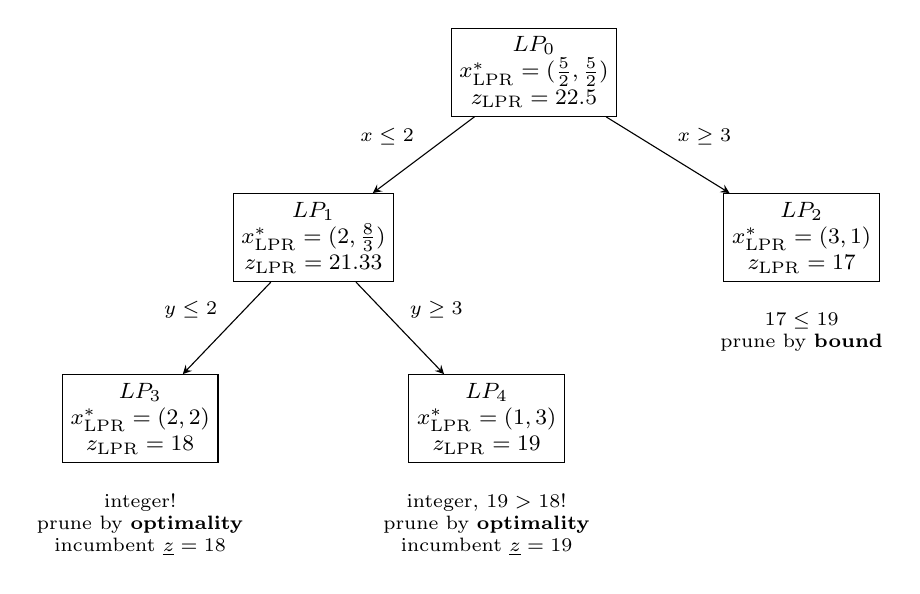
\begin{tikzpicture}[font=\small, >=stealth,
  bx/.style={draw, align=center, inner sep=3pt, font=\footnotesize}]
  \node[bx] (n0) at (0,0)       {$LP_0$\\ $x^{*}_{\mathrm{LPR}} = (\frac{5}{2}, \frac{5}{2})$\\ $z_{\mathrm{LPR}} = 22.5$};
  \node[bx] (n1) at (-2.8,-2.1) {$LP_1$\\ $x^{*}_{\mathrm{LPR}} = (2, \frac{8}{3})$\\ $z_{\mathrm{LPR}} = 21.33$};
  \node[bx] (n2) at (3.4,-2.1)  {$LP_2$\\ $x^{*}_{\mathrm{LPR}} = (3, 1)$\\ $z_{\mathrm{LPR}} = 17$};
  \node[bx] (n3) at (-5.0,-4.4) {$LP_3$\\ $x^{*}_{\mathrm{LPR}} = (2, 2)$\\ $z_{\mathrm{LPR}} = 18$};
  \node[bx] (n4) at (-0.6,-4.4) {$LP_4$\\ $x^{*}_{\mathrm{LPR}} = (1, 3)$\\ $z_{\mathrm{LPR}} = 19$};

  \draw[->] (n0) -- node[above left,  font=\scriptsize] {$x \le 2$} (n1);
  \draw[->] (n0) -- node[above right, font=\scriptsize] {$x \ge 3$} (n2);
  \draw[->] (n1) -- node[above left,  font=\scriptsize] {$y \le 2$} (n3);
  \draw[->] (n1) -- node[above right, font=\scriptsize] {$y \ge 3$} (n4);

  \node[align=center, font=\scriptsize] at (3.4,-3.3)
    {$17 \le 19$\\ prune by \textbf{bound}};
  \node[align=center, font=\scriptsize] at (-5.0,-5.75)
    {integer!\\ prune by \textbf{optimality}\\ incumbent $\underline{z} = 18$};
  \node[align=center, font=\scriptsize] at (-0.6,-5.75)
    {integer, $19 > 18$!\\ prune by \textbf{optimality}\\ incumbent $\underline{z} = 19$};
\end{tikzpicture}
\end{center}
\textbf{root.} \ solve $LP_0$ (drop integrality): $x^{*}_{\mathrm{LPR}} = (\frac{5}{2}, \frac{5}{2})$, $z_{\mathrm{LPR}} = 22.5$ --- fractional $\Rightarrow$ \textbf{branch}
\vspace{1pt}

\textbf{branch.} \ $x \le 2$ \ or \ $x \ge 3$: \ a decomposition (\S 4) that cuts out the fractional $x = 2.5$ and keeps every integer point
\begin{center}
\begin{tabular}{@{}lll@{}}
 $LP_1 = LP_0 + \{x \le 2\}$ & $x^{*}_{\mathrm{LPR}} = (2, \frac83)$, \ $z_{\mathrm{LPR}} = 21.33$ & fractional $\Rightarrow$ branch on $y$ \\[2pt]
 $LP_3 = LP_1 + \{y \le 2\}$ & $x^{*}_{\mathrm{LPR}} = (2,2)$, \ $z_{\mathrm{LPR}} = 18$ & integer $\Rightarrow$ prune by \emph{optimality}; \ incumbent $\underline{z} = 18$ \\[2pt]
 $LP_4 = LP_1 + \{y \ge 3\}$ & $x^{*}_{\mathrm{LPR}} = (1,3)$, \ $z_{\mathrm{LPR}} = 19$ & integer $\Rightarrow$ prune by \emph{optimality}; \ incumbent $\underline{z} = 19$ \\[2pt]
 $LP_2 = LP_0 + \{x \ge 3\}$ & $x^{*}_{\mathrm{LPR}} = (3,1)$, \ $z_{\mathrm{LPR}} = 17$ & $17 \le 19$ $\Rightarrow$ prune by \emph{bound} \ (integer, but cannot win) \\
\end{tabular}
\end{center}
no active problems remain $\Rightarrow$ stop. \ $z_{\mathrm{IP}} = 19$ at $(1,3)$ --- week 1's answer, now \textbf{proved}, with five LPs instead of enumerating
\vspace{2pt}

\textbf{infeasibility?} \ no piece of this tree is empty. \ in the demo, tilt the objective to $c = (10,1)$: $LP_0$ moves to $(\frac{10}{3}, 0)$,
and the branch $x \ge 4$ is empty ($3 \cdot 4 > 10$) --- prune by infeasibility
\vspace{3pt}

\medskip
\textbf{Algorithm (Branch and bound)}
\begin{center}
\begin{tabular}{@{}l|p{0.77\textwidth}@{}}
 \textbf{1. initialise} &
  incumbent $\underline{z} = c^{\top}\hat{x}$ if a feasible $\hat{x}$ is known, else $\underline{z} = -\infty$; \
  active list $L = \{LP_0\}$ \\[3pt]
 \textbf{2. stop?} &
  if $L = \emptyset$: \ $\underline{z} = -\infty$ $\Rightarrow$ report \emph{infeasible}; \
  otherwise report $\hat{x}$ as \textbf{optimal} \\[3pt]
 \textbf{3. select} &
  take a problem $LP_k$ from $L$ (and remove it); solve it for $z_{\mathrm{LPR}}$ and $x^{*}_{\mathrm{LPR}}$ \\[3pt]
 \textbf{4. prune} &
  LP infeasible $\Rightarrow$ prune, go to 2 \hfill \emph{(by infeasibility)} \newline
  $z_{\mathrm{LPR}} \le \underline{z}$ $\Rightarrow$ prune, go to 2 \hfill \emph{(by bound)} \newline
  $x^{*}_{\mathrm{LPR}}$ integer $\Rightarrow$ $\hat{x} = x^{*}_{\mathrm{LPR}}$, $\underline{z} = z_{\mathrm{LPR}}$; prune, go to 2 \hfill \emph{(by optimality)} \newline
  otherwise ($x^{*}_{\mathrm{LPR}}$ fractional) $\Rightarrow$ go to 5 \\[3pt]
 \textbf{5. branch} &
  pick a fractional $x_j = v$ in $x^{*}_{\mathrm{LPR}}$ (the \emph{branching variable} --- there can be many to choose from); \
  add two children $LP_{m+1}, LP_{m+2}$ to $L$ ($LP_m$ = the last problem created), go to 2: \newline
  \quad $P_{m+1} = P_k \cap \{x : x_j \le \lfloor v \rfloor\}$, \quad $P_{m+2} = P_k \cap \{x : x_j \ge \lceil v \rceil\}$ \\
\end{tabular}
\end{center}
for \textbf{binary} IP branching is simpler: \ $x_j = 0$ \ or \ $x_j = 1$
\vspace{2pt}

every line is something you already had: \ step 3 is \S 1's $z_{\mathrm{IP}} \le z_{\mathrm{LPR}}$; \ step 4 is the three prune rules above;
\ step 5 is \S 4's decomposition
\vspace{3pt}

modern solvers do not only branch: they also add cuts at the nodes, tightening $P$ as they go --- \textbf{branch \& cut}, week 15
\end{board}
\takeaway{branch \& bound = divide (\S 4) + bound (\S 1) + throw away what cannot win (\S 5). three prune rules: optimality, bound, infeasibility. it never enumerates $X$; it accounts for it.}

\end{document}
